\documentclass{article}

\usepackage{amssymb,amsfonts,amsmath,amsthm}
\usepackage{mathtools}
\usepackage{bm}
\usepackage{bbold}
\usepackage{pgfplots}
\pgfplotsset{width=7cm,compat=1.8}
\usepackage[margin=60pt]{geometry}

% Codons
\newcommand{\e}{\text{e}}
\begin{document}

\begin{center}
	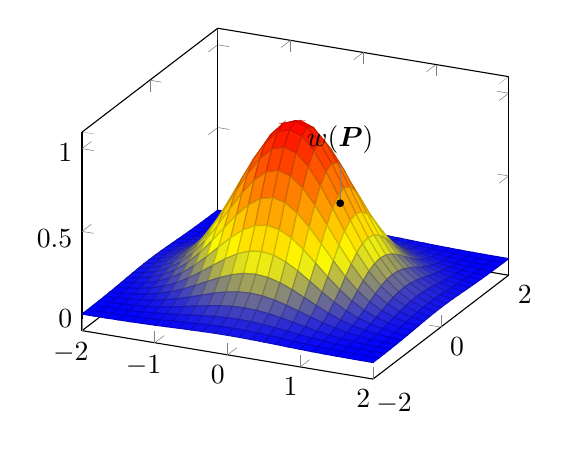
\begin{tikzpicture}
		\begin{axis}
		\addplot3[surf,domain=-2:2,domain y=-2:2] 
		{exp(-( x^2 + y^2) )};
		\node[circle,inner sep=1pt,fill=black,pin=90:$w(\bm{P})$] 
		at (axis cs:0.5,0.25,0.5) {};
		\end{axis}
	\end{tikzpicture}
\end{center}
\end{document}